\documentclass[a5paper,11pt]{article} %Le format A5, pratique à emporter
\usepackage[left=2.5cm,right=2cm,top=1cm,bottom=1.5cm,twoside=true]{geometry}
\usepackage{hyperref}
\hypersetup{
  bookmarks=true,
  bookmarksopen=true,
  unicode=true,
  pdftoolbar=true,
  pdfmenubar=true,
  pdftitle={FabLab de Pau},
  pdfauthor={PauLLA},
  colorlinks=true,
  linkcolor=black,
  urlcolor=black,
  pdftex=true,
  hyperindex=true  
}
\usepackage[T1]{fontenc}
\usepackage[utf8]{inputenc}
\usepackage{french}
\usepackage{marvosym}
\usepackage{graphicx}
\usepackage{garamondx}
\usepackage{url}

\title{FabLab de Pau} %Nom à revoir
\author{PauLLA -- C.D.A. Pau Porte des Pyrénées}

\begin{document}


%\maketitle\thispagestyle{empty}
%\pagebreak
\thispagestyle{empty}
\begin{center}

\includegraphics[width=0.15\textwidth]{paulla.png} \hfill 
\includegraphics[width=0.35\textwidth]{PPP.png}
\\~\\

\includegraphics[width=0.25\textwidth]{UPPA.png} \hfill 
\includegraphics[width=0.30\textwidth]{innovate.png}
\vfill
\Huge FabLab de Pau\\~\\
\huge Livret d'acceuil
\vfill
\footnotesize Version du 25 mai 2014
\end{center}

\pagebreak
~ \vfill % workaround pour centrer la table des matières...
\tableofcontents\thispagestyle{empty}
~ \vfill % workaround pour centrer la table des matières...
\pagebreak\section{Introduction}
Le FabLab de Pau, soutenue par la communauté d'agglomération de Pau\footnote{\texttt{http://www.pau.fr/}} et porté par l'association PauLLA\footnote{\texttt{http://www.paulla.asso.fr/}}, est un espace de fabrication numérique et de prototypage. On y retrouve des machines pilotées par ordinateur ainsi que du matériel permettant la création, l'étude  ou la modification de circuits électroniques. D'autres outils, comme des perceuses ou des machines à coudre peuvent êtres disponibles.

Le FabLab de Pau est également un lieu de rencontre entre créateurs, étudiants, artistes, ingénieurs, particuliers, professionnels, \dots 

Le présent livret a pour objectif de présenter rapidement le FabLab de Pau, ainsi que ses conditions particulières : charte des fablabs, règlement intérieur, horaires d'ouverture ou encore tarifs d'utilisations.

% Présentation en QQOQCCP, simple et complète

\subsection{L'équipe du FabLab}
\subsubsection{Les référents}
% Qui sont les référents, rôles etc
Il existe au sein du FabLab des personnes nommées référents.
Ce sont les référents qui ont en charge l'ouverture et la fermeture du local.
Certains référents sont spécialisés dans l'utilisation et la maintenance d'une ou plusieurs machines.
Les référents sont garants du respect des conditions d'utilisation du FabLab (réglemenent intérieur et charte des fablabs).
Les référents peuvent à leurs tours former d'autres référents.
La liste des référents, leurs aptitudes ainsi que leurs temps de présence au FabLab est disponible sur le site internet du FabLab. %Il faudrait mettre un lien dès que possible : \footnote{\texttt{http://lien}}

\subsubsection{Les partenaires}
% partenaires = personnes morales avec convention paulla ?
Les partenaires sont des structures, par exemple des associations ou des entreprises, ayant signé une convention avec PauLLA pour l'utilisation du FabLab.
Ces partenaires peuvent avoir en leur sein un (ou plusieurs) référent, ce qui leur permet d'utiliser le FabLab en toute autonomie.

\subsection{Horaires d'ouverture}
%Insérer un planning type + ref au site ? adresse simple ? ical/vcal ?
Il existe plusieurs types de plages horaires d'ouverture possible au FabLab : les plages reservées pour le projet d'un partenaire, les plages dédiées à un thème, un atelier, ou une formation (en partenariat avec la cyberbase Pau~-~Pyrénnées), et les plages d'ouverture sans objectif prédéfini.
Le FabLab est toujours ouvert au public, dans le respect du réglement intérieur, y compris durant les temps "reservés". Néanmoins, l'accès aux machines ne peut être garanti, quelques projets demandant parfois plusieurs heures de temps machine-outil.
Comme spécifié dans le réglement intérieur, le FabLab est succeptible d'être ouvert à toute heure du jour ou de la nuit, n'importe quel jour de l'année.
L'agenda détaillé d'ouverture est disponible sur le site internet du FabLab. %Il faudrait mettre un lien dès que possible : \footnote{\texttt{http://lien}}

\subsection{Lieu}
Le FabLab de Pau est situé 4 rue Despourrins, à Pau, au dessus de la cyberbase. Non loin du centre ville
%Ajouter les accès bus, parking bosquet, attache vélo près de la porte de la cyberbase 
%Une photo ?
\subsection{Que fait-on au FabLab ?}
%Oui, oui, on bricole...
\subsection{Comment fonctionne le FabLab ?}

\subsection{Les tarifs du FabLab}
% Trésorier, je compte sur toi pour cette section

\subsubsection{Utilisation des machines}

\subsection{Pourquoi venir au FabLab ?}
%Motivons les à venir !

\pagebreak\section{Charte du FabLab}
%http://www.paulla.asso.fr/intranet/relations-avec-partenaires/cda-pau-porte-des-pyrenees/fablab-hackerspace/fonctionnement-pratique-du-fablab/reglement-interieur-work-in-progress
{\small \begin{center}
La version originale est disponible sur le site du M.I.T. : \\ \texttt{http://fab.cba.mit.edu/about/charter/}
\end{center}}
\begin{description}
  \item[Qu'est-ce qu'un FabLab ?]
On désigne sous le nom FabLab un réseau global de laboratoires locaux permettant la création ou fabrication à travers la mise à disposition d'outils de fabrication numériques.

\item[Que trouve-t-on dans un FabLab ?]
Les FabLab proposent un panel d'outils de base permettant de tout fabriquer (ou presque) tout en facilitant le partage des connaissances au sein de ses utilisateurs.

\item[Que propose le réseau des FabLab ?]
Une assistance opérationnelle, éducative, technique, financière et logistique qui va au-delà de ce qu'un seul laboratoire est en mesure de proposer.

\item[Qui peut utiliser les services d'un FabLab ?]
Les FabLab constituent une ressource collective, offrant un accès libre pour les individus ainsi qu'un planning d'activités.

\item[De quoi êtes vous responsable en tant qu'utilisateur ?]
La sécurité : ne rien faire qui puisse blesser un autre utilisateur, vous même ou endommager un outil
Le bon fonctionnement : participer au nettoyage, à la maintenance et tout faire pour améliorer le laboratoire
Le partage des connaissances : contribuer à documenter et enseigner
 

\item[A qui appartiennent les idées issues du FabLab ?]
Les procédés et créations développés au sein d'un FabLab peuvent être protégés et vendus selon la volonté de leur auteur, mais devraient rester libre d'accès au plus grand nombre afin d'en permettre l'usage et l'étude.

\item[De quelle manière une entreprise peut-elle disposer d'un FabLab ?]
Les activités commerciales peuvent être créées et développées au sein d'un FabLab, mais elle ne doivent pas entrer en conflit avec ses autres activités, elles devraient plutôt se développer à l'extérieur plutôt qu'à l'intérieur du laboratoire et bénéficier au créateurs, laboratoires et réseaux qui ont permis leur succès.
\end{description}
% \vfill
% \begin{center}
%   
\includegraphics[width=0.25\textwidth]{fablab-logo.png}
% \end{center}
% \vfill

\pagebreak\section{Règlement intérieur}
%http://www.paulla.asso.fr/intranet/relations-avec-partenaires/cda-pau-porte-des-pyrenees/fablab-hackerspace/fonctionnement-pratique-du-fablab/reglement-interieur-work-in-progress

\subsection*{Article 1. Préambule}
Le FabLab est un lieu ouvert situé à Pau. Il se trouve 4 rue Despourrins, au premier étage, et est géré par l'association PauLLA. Son objectif est d'être un "Laboratoire de Fabrication" qui s'inscrit dans le cadre défini par le M.I.T (\textit{Massachussetts Institute of Technology}) dans la charte du même nom.
Le présent règlement, rédigé et validé par l'association PauLLA, fixe les droits et obligations des usagers du FabLab. Les représentants de l'association sont chargés de le faire appliquer.

\subsection*{Article 2. Champ d'application}
Quiconque souhaite fréquenter le FabLab s'engage à accepter les articles du présent règlement qui s'applique à toute personne présente dans son enceinte et/ou dans les activités qui pourraient être organisées à l'extérieur.

\subsection*{Article 3. Conditions d'accès}
\subsubsection*{Section 3.1 Horaires}
Le FabLab est susceptible d'être ouvert à n'importe quelle heure de la journée entre 0h et 23h59 du 1er janvier au 31 décembre. Les créneaux d'ouverture sont annoncés sur son site internet, via son compte Twitter, sur son canal IRC et toute autre solution technique que l'association PauLLA jugera utile de mettre en place.
\subsubsection*{Section 3.2 Tarifs}
L'accès au FabLab est gratuit. Les tarifs liés à l'utilisation des machines, aux consommables, à la participation à certaines animations spécifiques sont affichés dans le local et sur le site internet. Ils sont fixés par l'association PauLLA et peuvent être révisés sans preavis.
\subsubsection*{Section 3.3 Accès des mineurs}
Les mineurs souhaitant fréquenter le FabLab doivent obtenir l'autorisation d'un représentant légal. Les enfants de moins de 12 ans devront systématiquement être accompagnés d'un adulte. Pour la participation aux activités, ils devront être amenés et récupérés par la même personne.

\subsection*{Article 4. Fonctionnement}
\subsubsection*{Section 4.1 Les référents}
Lorsque le FabLab est ouvert, les référents de l'association PauLLA sont à la disposition des usagers pour renseigner à propos du fonctionnement du lieu, initier à l'utilisation des machines, échanger des connaissances... etc.
\subsubsection*{Section 4.2 Accès aux machines}
Certaines machines mises à la disposition des utilisateurs peuvent présenter un danger si elles sont mal utilisées. Les personnes désirant les utiliser sont invitées à respecter les consignes affichées à proximité. En cas de doute, ils sont tenus de s'adresser à un référent.

\subsection*{Article 5. Règles générale d'utilisation}
\subsubsection*{Section 5.1 Interdictions}
Il est interdit aux usagers :
\begin{itemize}
  \item De fumer et de vapoter dans le local.
  \item De manger et de boire en dehors de la zone prévue à cet effet
  \item De se mettre en danger ou de mettre en danger les autres utilisateurs par une utilisation inappropriée des outils mis à leur disposition
\end{itemize}
\subsubsection*{Section 5.2 Comportement des usagers}
Les usagers sont tenus de respecter le calme à l'intérieur des locaux et d'y avoir une tenue correcte. Ils ne devront en aucun cas être cause de nuisances pour les autres usagers et les référents.
Les effets personnels des usagers sont placés sous leur propre responsabilité.
Toute dégradation des locaux ou du matériel, tout vol, pourra entraîner des sanctions internes et/ou une poursuite judiciaire impliquant notamment la réparation du dommage.
Toute agression physique ou verbale à l'encontre des référents pourra faire l'objet d'une plainte.
\subsubsection*{Section 5.3 Hygiène et sécurité}
Il est interdit de pénétrer ou de demeurer dans le FabLab en état d'ébriété ou sous l'emprise de drogues.
L'accès des animaux est interdit dans le Fablab à l'exception des animaux guides.

\subsection*{Article 6. Limitation du droit d'usage}
Les référents du FabLab sont chargés de mettre en œuvre les moyens techniques et humains visant à faire appliquer le présent règlement sous l'autorité du Président de l'association PauLLA.
Le non-respect d'une ou plusieurs des consignes énoncées ci-dessus entraînera les sanctions suivantes :
\begin{itemize}
  \item éviction des lieux sur le champ
  \item interdiction temporaire ou définitive d'accès au FabLab
\end{itemize}

\subsection*{Article 7. Modification du présent règlement}
Le présent règlement pourra être modifié à tout moment, les modifications s'appliqueront de plein droit à tout usager.

\pagebreak\section{Fiche projet type}
\paragraph{Au départ}
\begin{itemize}
  \item Nom du projet : 
  \item Auteur(s) : 
  \item Description succincte : [quelques lignes descriptives du projet tel que son auteur l'imagine]
  \item Date de début :
  \item Date de fin estimée : 
\end{itemize}
\paragraph{Projet en cours}
~\\
Statut du projet : Démarrage / En cours de réalisation / Terminé / Abandonné
\subparagraph{Réalisation : }
\textit{Veuillez détailler ici les grandes étapes de la réalisation, en tous cas ce qui est fait au FabLab. Ne pas lésiner sur la quantité de texte et de photos.
Merci de mettre en ligne les fichiers permettant à d'autres utilisateurs de reprendre le projet en cours ou de le réaliser à l'identique en précisant les logiciels utilisés.
La liste des outils et machines ayant permis au projet de se faire est également la bienvenue.
Si votre projet est basé sur une réalisation existante, merci d'en indiquer les références (lien web, article de presse\dots).}

\paragraph{Projet terminé}
~\\
Date de fin réelle : \\
\textit{Le projet que vous avez mené :
\begin{itemize}
  \item est-il arrivé à son terme ?
  \item le résultat final correspond-il à ce qui a été envisagé au départ ?
  \item veuillez indiquer une estimation du temps passé
  \item avez-vous trouvé au FabLab tous les outils permettant de mener à bien votre projet ? Si la réponse est non, qu'est-ce qui vous a manqué ?
  \item avez-vous eu l'occasion d'échanger des connaissances / des bonnes pratiques / des idées nouvelles avec les autres utilisateurs du FabLab ?
\end{itemize}}

\pagebreak\section{Contact}
\begin{center}
  \vfill
  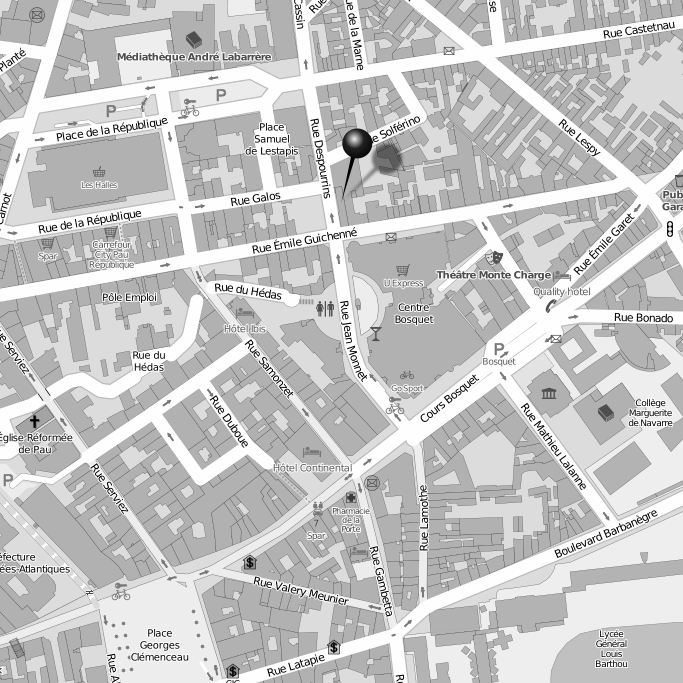
\includegraphics[width=10cm]{carte.png}
  \vfill
  FabLab\\
  4 Rue Despourrins\\
  64000 Pau\\
  \vfill
  \medskip Téléphone : 05.32.09.04.76\\ %\Telefon
  \medskip E-mail : \href{mailto:paulla@inbricolewetrust.net}{\texttt{paulla@inbricolewetrust.net}}\\%\MVAt
  \medskip Site web : \url{http://paulla.inbricolewetrust.net/}\\%\Keyboard
  \medskip Twitter : \href{https://twitter.com/FabLab}{\texttt{@FabLab}}
  \vfill
\end{center}

\end{document}
